\begin{figure*}[tb]
    \begin{subfigure}{0.49\textwidth}
        \centering
        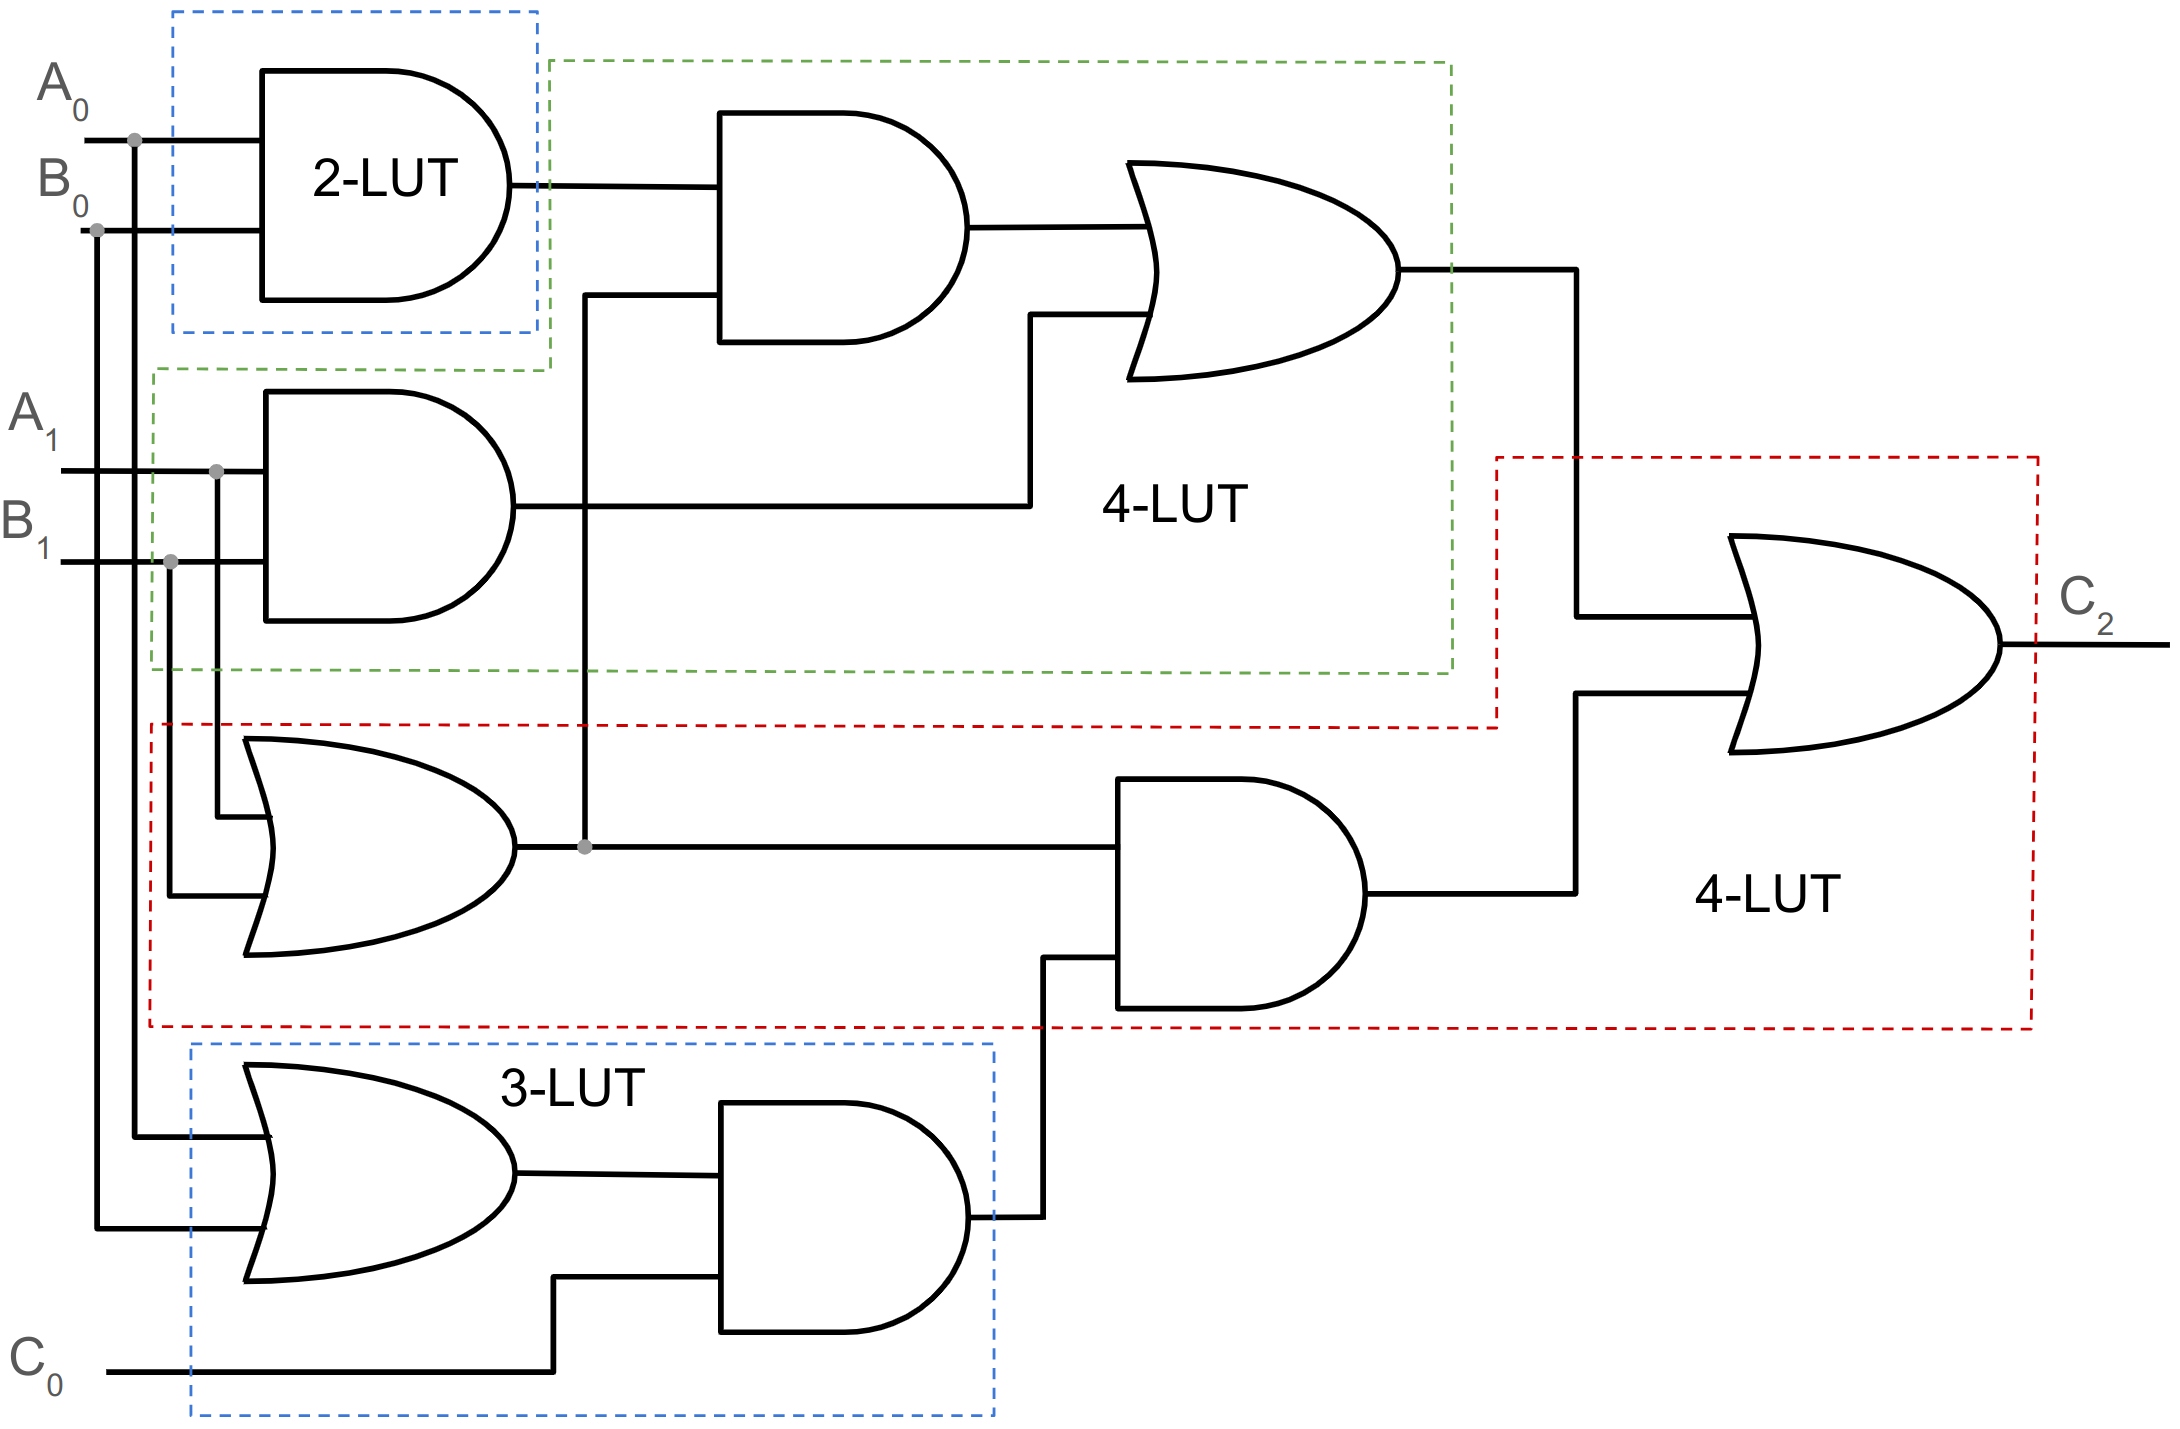
\includegraphics[width=0.92\textwidth]{img/cla_bad.png}
        \caption{An implementation that uses four LUTs contains redundancy.}\label{fig:eg:bad}
    \end{subfigure}
    \hfill
    \begin{subfigure}{0.49\textwidth}
        \centering
        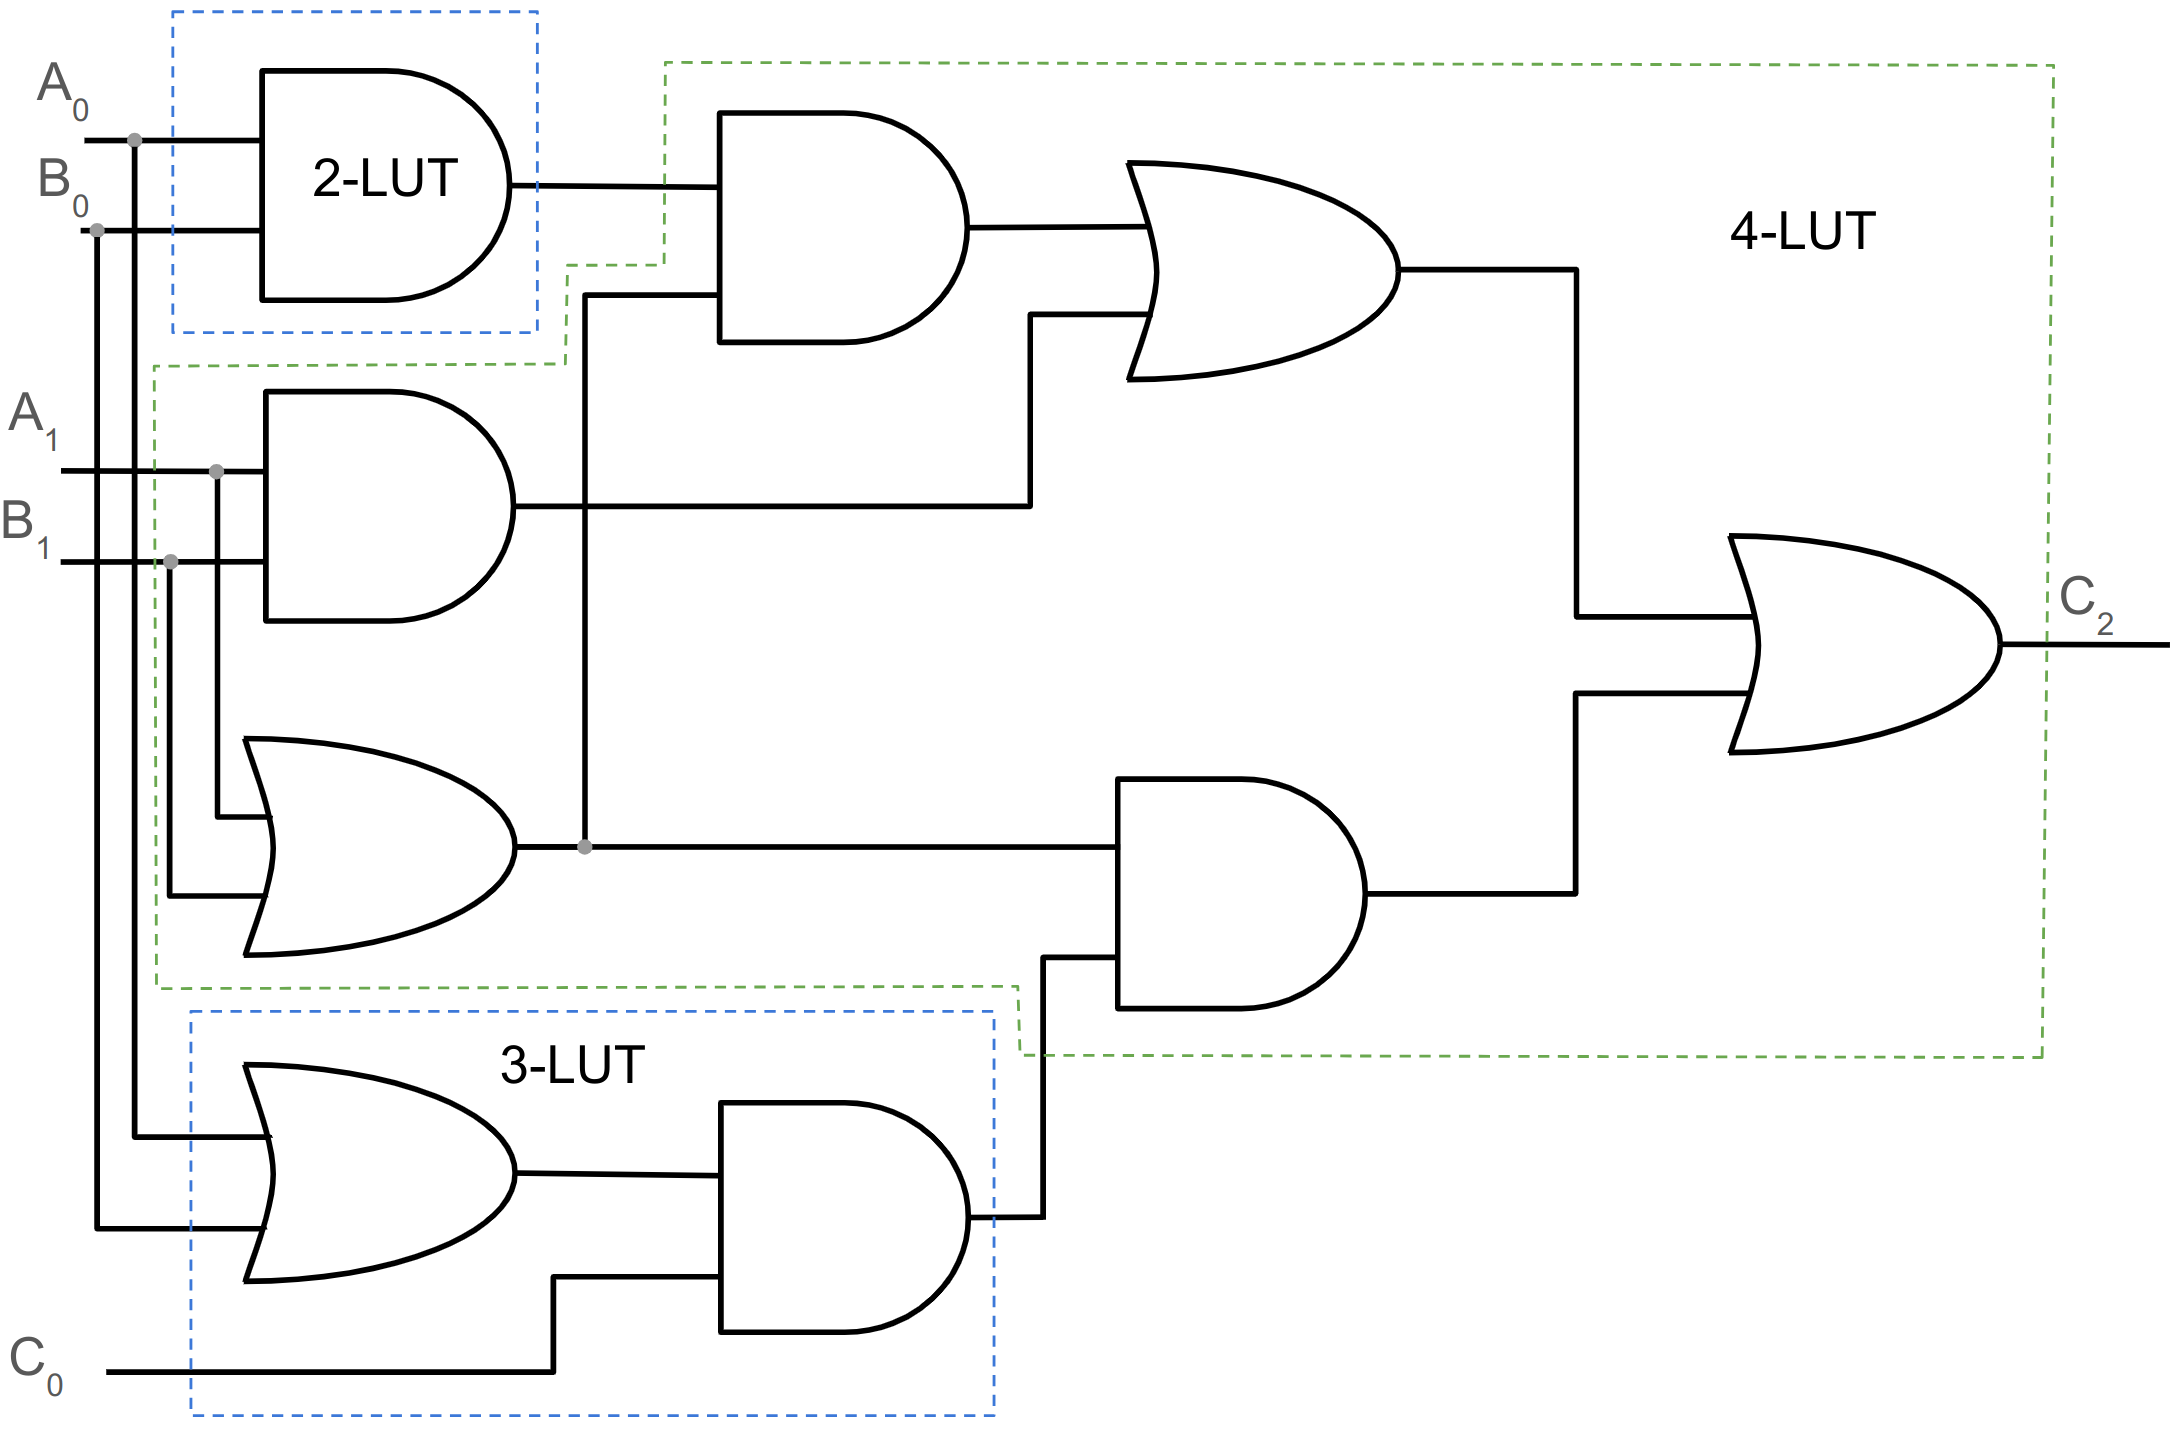
\includegraphics[width=0.92\textwidth]{img/cla_good.png}
        \caption{The sink cut of logic can expand its cover and reduce the LUT count by one.}\label{fig:eg:good}
    \end{subfigure}
    \caption{2-bit CLA (carry-lookahead) demonstrates that non-monotone clustering can map suboptimally to a 4-LUT FPGA.}\label{fig:eg}
\end{figure*}

\section{Background}\label{sec:background}

\subsection{FPGA Technology Mapping}\label{sec:background:fpga}
FPGA technology mapping converts abstract RTL logic into a netlist of lookup
tables (LUTs). Due to the computational complexity of optimal LUT packing, most
implementations avoid restructuring the input logic and are essentially graph
covering algorithms. Given a $k$-LUT FPGA architecture, most mappers start by
enumerating the feasible cuts of logic for each node in the circuit. Where
competing implementations vary, however, is the set of heuristics they use to
map logic cuts to LUTs. Cut selection essentially decides the graph covering to
use. As an example, Fig.~\ref{fig:eg} shows differing results of mapping
carry-lookahead logic to FPGA LUTs.
% Flow map uses two passes

\subsection{Equivalence Graphs}\label{sec:background:egraph}
Equivalence graphs (e-graphs) are a data structure originally conceived to
facilitate automated proof generation~\cite{eggpaper, eqsat}. For example,
e-graphs can be used to rewrite mathematical expressions~\cite{egraphmath} or
for automated reasoning about functional programs~\cite{cclemma}.

Equality saturation is useful for optimizing compilers, because it defers
greedy program transformations. Extracting solutions from saturated e-graphs
can result in more optimal---sometimes provably optimal---programs. In
contrast, traditional compilers use a pass pipeline architecture which suffers
from a \textit{phase-ordering problem}. In other words, there is never an
ordering of transformation passes that is optimal for all input programs. This
is a deep-rooted issue in compiler design, but the problem is particularly
consequential for hardware design.
